
\documentclass[conference]{IEEEtran}
\usepackage{blindtext, graphicx}
\usepackage[utf8]{inputenc}
\usepackage[spanish, activeacute]{babel} 
\usepackage{listings}
\usepackage{amssymb}
\usepackage[breaklinks=true]{hyperref}
\pagestyle{myheadings}
\markright{Estrategias de seguridad en base de datos}
\hyphenation{op-tical net-works semi-conduc-tor}

\begin{document}

\title{ESTRATEGIAS DE SEGURIDAD EN BASE DE DATOS}
% make the title area
\maketitle


\begin{abstract}
Es indudable que cada dia las entidades dependen de mayor medida de la información y de la tecnologia, y que los sistemas de información están más soportadas por la tecnologia, frente a la realidad de hace pocas décadas.
\\
Por otra parte, hace unos años la protección era más facil,con arquitecturas centralizadas y terminales no inteligentes , pero hoy en día los entornos son realmente complejos, con diverdidad de plataformas y proliferación de redes, no sólo internas sino también externas, incluso con enlaces internacionales.
\\
Entre las plataformas físicas (hardware) pueden estar: ordenadores grandes y medios ordenadores departamentales y personales, solos o formando parte de red, e incluso ordenadores portátiles. Esta diversidad acerca la información a los usuarios, si bien hace mucho más dificil proteger los datos, especialmente porque los equipos tienen filosofias y sistemas operativos diferentes, incluso a veces siendo del mismo fabricante.
\\
Al hablar de seguridad hemos preferido centrarnos en la información misma, aunque a menudo se hable de seguridad informatica, de seguridad de los sistemas de información o de seguridad de las tecnologias de la información.
\\
En cualquier caso hay tres aspectos principales, como distintas vertientes de la seguridad.
\\
\end{abstract}

\begin{abstract}

Undoubtedly, every day the entities depend more on information and technology, and that information systems are more supported by technology, compared to the reality of a few decades ago.
\\
On the other hand, a few years ago the protection was easier, with centralized architectures and non-intelligent terminals, but nowadays the environments are really complex, with divergence of platforms and proliferation of networks, not only internal but also external, even with links international
\\
Among the physical platforms (hardware) can be: large computers and departmental and personal computers, alone or as part of the network, and even laptops. This diversity brings information closer to users, although it makes it much more difficult to protect data, especially because computers have different philosophies and operating systems, sometimes even from the same manufacturer.
\\
When talking about security, we have preferred to focus on the information itself, although there is often talk about information security, security of information systems or security of information technologies.
\\
In any case there are three main aspects, as different aspects of security.
\end{abstract}

% Note that keywords are not normally used for peerreview papers.
\begin{IEEEkeywords}
seguridad base de datos, MySQL, MongoDB.
\end{IEEEkeywords}


\IEEEpeerreviewmaketitle


\section{Introducci\'on}
La gran mayoría de los datos sensibles del mundo están almacenados en sistemas gestores de bases de datos comerciales tales como Oracle, Microsoft SQL Server entre otros, atacar una bases de datos es uno de los objetivos favoritos para los criminales.
\\
Esto puede explicar por qué los ataques externos, tales como inyección de SQL, subieron 345 por ciento en 2009, “Esta tendencia es prueba adicional de que los agresores tienen éxito en hospedar páginas Web maliciosas, y de que las vulnerabilidades y explotación en relación a los navegadores Web están conformando un beneficio importante para ellos”[*]
\\
Para empeorar las cosas, según un estudio publicado en febrero de 2009 The Independent Oracle Users Group (IOUG), casi la mitad de todos los usuarios de Oracle tienen al menos dos parches sin aplicar en sus manejadores de bases de datos [1].
\\
 Mientras que la atención generalmente se ha centrado en asegurar los perímetros de las redes por medio de, firewalls, IDS / IPS y antivirus, cada vez más las organizaciones se están enfocando en la seguridad de las bases de datos con datos críticos, protegiéndolos de intrusiones y cambios no autorizados
\\
En las siguientes secciones daremos las siete recomendaciones para proteger una base de datos en instalaciones tradicionales..
\\

\section{CONCEPTO}

La seguridad en las base de datos es un mecanismo fundamental ya que todo de sistema informatizado esta expuesto a cualquier tipo de amenazas de daño, enormes y desastrosas como pequeñas y leves pero que de una manera u otra causan perdida de confidencialidad
\\
\begin{flushright}
  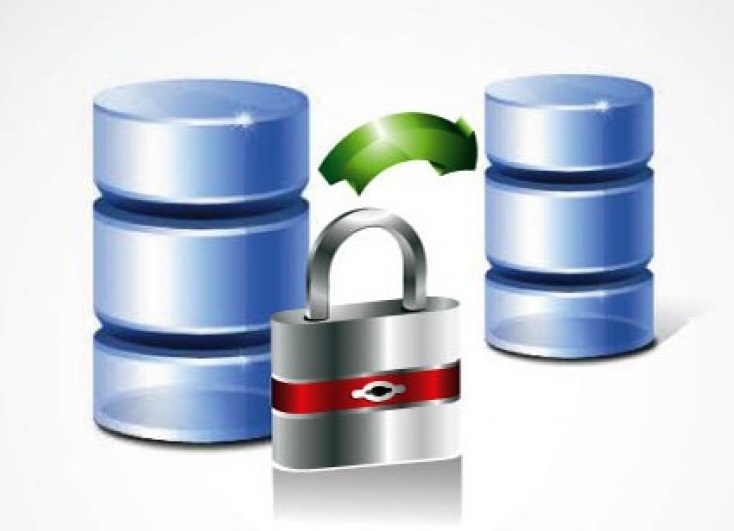
\includegraphics[scale=0.31]{Imagenes/seguridadbd.jpg}
\end{flushright}
\centering
\\Figura 1
\\

\begin{itemize}
\item \textbf{AMENAZAS:} Se deben considerar las amenazas para cada tipo de empresa donde se implementara el sistema de base de datos, ya que pueden haber amenazas particulares a las que se este mas expuesto.
\end{itemize}

\section{PRINCIPIOS BÁSICOS PARA LA SEGURIDAD}

\begin{itemize}
\item \textbf{}Identifique su sensibilidad 
\item \textbf{}Evaluación de la vulnerabilidad y la configuración 
\item \textbf{}Endurecimiento 
\item \textbf{}Audite 
\item \textbf{}Monitoreo 
\item \textbf{}Pistas de Auditoría 
\item \textbf{}Autenticación, control de acceso, y Gestión de derechos
\end{itemize}
\section{MEDIDAS DE SEGURIDAD}

Suponer que el diseño del sistema es público:
\begin{itemize}
\item \textbf{FÍSICAS:} Controlar el acceso al equipo.
\\
mediante tarjetas de acceso.
\item \textbf{PERSONAL:} Acceso solo de personal autorizado.
\\
identificación directa de personal.
\item \textbf{SGBD:} Uso de herramientas que proporcione el SGBD.
\\
perfiles de usuario, vistas, restricciones de uso de vistas.
\\
\end{itemize}
\\

\section{REQUISITOS PARA LA SEGURIDAD DE LAS BD}
\begin{itemize}
\item \textbf{} La base de datos debe ser protegida contra el fuego, el robo y otras formas de destrucción.
\\
\item \textbf{} Los datos deben ser reconstruibles, ya que siempre pueden ocurrir accidentes.
\\
\item \textbf{} Los datos deben poder ser sometidos a procesos de auditoria.
\\
\item \textbf{} El sistema debe diseñarse a prueba de intromisiones, no deben poder pasar por alto los controles.
\\
\item \textbf{} Ningún sistema puede evitar las intromisiones malintencionadas, pero es posible hacer que resulte muy difícil eludir los controles.
\\
\item \textbf{} El sistema debe tener capacidad para verificar que sus acciones han sido autorizadas
\\
\item \textbf{} Las acciones de los usuarios deben ser supervisadas, de modo tal que pueda descubrirse cualquier acción indebida o errónea.
\\
\end{itemize}

\section{CARACTERÍSTICAS PRINCIPALES}
El objetivo es proteger la Base de Datos contra
accesos no autorizados.
Las 3 principales caracteristicas de la seguridad en la base de datos son:
\begin{itemize}
\item \textbf{}La Confidencialidad de la información.
\item \textbf{}La Integridad de la información.
\item \textbf{}La Disponibilidad de la información.
\end{itemize}
\\

\section{ANALISIS}
Qué es la seguridad de la información y qué tiene que ver con la integridad en base de datos.
La seguridad de la información se ocupa de proteger la confidencialidad, disponibilidad e integridad en base de datos de todos los activos de conocimiento de la organización. La forma de lograrlo tiene que ver con:
\begin{itemize}
\item \textbf{}Confidencialidad: se trata del aspecto más importante de la seguridad de base de datos. Este objetivo se alcanza a través del La encriptación ha de aplicarse a datos en reposo, pero también a los datos que, por un motivo u otro, se encuentren en tránsito.
\item \textbf{}Integridad en base de datos: busca garantizar que sólo las personas autorizadas a ello podrán acceder a información privilegiada de la empresa. La integridad de una base de datos se aplica a través de protocolos de autenticación, políticas internas (como las que impulsan la seguridad de las contraseñas) y un sistema de control de acceso de usuario que define los permisos que determinan quién puede acceder a qué datos. Tampoco puede olvidarse el tomar medidas que ayuden a conseguir que las cuentas no utilizadas queden bloqueadas o sean eliminadas.
\item \textbf{}Disponibilidad: hace referencia a la necesidad de que las bases de datos y toda la información que contienen estén listas para su uso. Por una parte, se debe garantizar su funcionalidad y confiabilidad mientras que, por otra, es recomendable planificar los tiempos de inactividad fuera del horario laboral.
\end{itemize}
\\

\section{TECNICAS DE SEGURIDAD}
El mecanismo de seguridad de un SGBD3 debe incluir formas de restringir el acceso al sistema como un todo. Ésto, se denomina control de acceso y se pone en practicas creando cuentas de usuarios y contraseñas para que es SGBD controle el proceso de entrada al sistema.Otra técnica de seguridad es el cifrado de datos, que sirve paraproteger datos confidenciales que se transmiten por satélite o por algún otro tipo de red de comunicaciones. El cifrado provee protección adicional a secciones confidenciales de una base de datos. Los datos se codifican mediante algún algoritmo ex profeso. Un usuario no autorizado que tenga acceso a los datos codificados tendrá problemas para descifrarlos, pero un usuario autorizado contará con algoritmos (o claves) de codificación o descifrado para tal efecto. 


\begin{itemize}
\item \textbf{Cl administrador de la base de datos: }Es la autoridad central que controla un sistema de este tipo. El DBA4 tiene una cuenta privilegiada en el SGBD, a veces denominada cuenta del sistema, que confiere capacidades extraordinarias no disponibles para cuentas y usuarios ordinarios de la base de datos. El DBA ejecuta los siguientes tipos de acciones:
\item \textbf{} Creación de cuentas.
\item \textbf{}Concesión de privilegios.
\item \textbf{}Revocación de privilegios.
\item \textbf{}Asignación de niveles de seguridad.
\item \textbf{}Es el responsable de la seguridad global del sistema de base de datos.


\item \textbf{Integridad en base de datos:} busca garantizar que sólo las personas autorizadas a ello podrán acceder a información privilegiada de la empresa. La integridad de una base de datos se aplica a través de protocolos de autenticación, políticas internas (como las que impulsan la seguridad de las contraseñas) y un sistema de control de acceso de usuario que define los permisos que determinan quién puede acceder a qué datos. Tampoco puede olvidarse el tomar medidas que ayuden a conseguir que las cuentas no utilizadas queden bloqueadas o sean eliminadas.
\item \textbf{Disponibilidad:} hace referencia a la necesidad de que las bases de datos y toda la información que contienen estén listas para su uso. Por una parte, se debe garantizar su funcionalidad y confiabilidad mientras que, por otra, es recomendable planificar los tiempos de inactividad fuera del horario laboral.
\end{itemize}
\\
\section{CONTROLES INFORMATIZADOS PARA ENTORNOS MULTIUSUARIOS}
\subsection{Autorizacion}
Autorización es como el poder administrativo que se necesita para acceder legítimamente a un sistema.
\subsection{La autenticacion}
La autenticación es la validación de identidad del usuario.

\section{SEGURIDAD EN BASE DE DATOS}
\begin{itemize}
\item \textbf{Controles de acceso:}
Existen dos tipos de controles: 
\item \textbf{Control de accesos discrecional (DAC): } emplea un mecanismo de SQL conocido con el nombre de control de accesos discrecional.
\item \textbf{Control de acceso obligatorio (MAC):}
se basa en políticas de nivel de sistema que no pueden ser modificadas por usuarios individuales.
\item \textbf{Vistas:}
Este mecanismo de vistas proporciona un sistema de seguridad potente y flexible, al ocultar partes de la base de datos a ciertos usuarios. 
Son relaciones virtuales que no existen en realidad en la base de datos.

\item \textbf{Copias de seguridad: }
Tener respaldos de la BD actualizados para cuando se produzcan errores de perdida de datos,  para garantizar la integridad física de los datos.
\item \textbf{Integridad: }
La seguridad en un SGDB se trata de impedir la distorsión de la DB, mediante esta se pretende proteger la base de datos contra operaciones que introduzcan inconsistencias en los datos
\item \textbf{Cifrado: }
Es ocultar los caracteres legibles de una clave.

\item \textbf{Tecnología RAID Matriz redundante de discos independientes: }
Es un tipo de tecnología que se lo establece para que funcione redundantemente en los fallos que se vaya presentando.

\item \textbf{SEGURIDAD EN SGBD DE MICROSOFT OFFICE ACCESS: }
Se basa en la configuración de una contraseña general para los diferentes usuarios y un permiso a nivel de privilegios para cada usuario

\item \textbf{EN SGBD DE ORACLE: }
Entre los privilegios que pueden accederse en Oracle estarían los derechos a: Conectarse a la base de datos (crear una sesión), Crear una tabla.
\item \textbf{Seguridad de un SGBD en entornos web: }
Debemos incluir para este tipo de seguridad: los servidores proxy, cortafuegos, algoritmos de compendio de mensajes y firmas digitales, certificados digitales, kerberos, Secure Sockets Layer (SSL) y secure HTTP (S-HTTP), secureelectronicTransactions (SET), etc.


\end{itemize}

\section{Conclusiones}
  La base de datos a hecho avances significativos en el manejo de la seguridad de las bases de datos.
  \\
  Varias de las aplicaciones que manejamos en nuestro diario vivir que requieren confidencialidad necesitan modelos mas sofisticados de seguridad: Entidades bancarias, medicas, departamentos gubernamentales, inteligencia militar, etc.
  \\
  Aunque la implementación de seguridad mas sofisticada no es tarea fácil, debemos hacer el esfuerzo por lograr que nuestros datos estén completamente seguros


\ifCLASSOPTIONcaptionsoff
  \newpage
\fi


\begin{thebibliography}{1}

\bibitem{SeguridadTecnologica}
ISO/IEC 27001:2005 - Information technology -- Security    techniques [en]
\\
http://www.iso.org/iso/catalogue-detail?Csnumber=42103.

\bibitem{sistemaAlmacenamiento}
Pramod J. Sadalage Martin Fowler. NoSQL Distilled: A brief Guide to the Emerging
World of Polyglot Persistence. Addison-Wesley, 2013.

\bibitem{BigTable}
Fay Chang, Jeffrey Dean, Sanjay Ghemawat, Wilson C. Hsieh, Deborah A. Wallach, Mike Burrows, Tushar Chandra, Andrew Fikes, and Robert E. Gruber. 2008. Bigtable: A Distributed Storage System for Structured Data. ACM Trans. Comput. Syst. 26, 2, Article 4 (June 2008), 26 pages. DOI=http://dx.doi.org/10.1145/1365815.1365816

\bibitem{NoSQL}
Vaish, Gaurav. Getting Started with NoSQL. Packt Publishing, 2013.

\bibitem{Json}
ECMA-404. Introducción a JSON. 2013. [online]
Disponible en: http://www.json.org/json-es.html

\bibitem{wanderu}
Boyd R. Polyglot Persistence Case Study: Wanderu + Neo4j + MongoDB Neo4j Blog, 2015.

\bibitem{zephyr}
Chaudhari M. Integrating Diverse Healthcare Data using MongoDB and Neo4j.Neo4j Blog, 2016.

\bibitem{mongo}
MongoDB, Inc. Reinventando la gestión de datos. [online]
Disponible en: https://www.mongodb.com/es

\bibitem{neo}
Neo Technology, Inc. Neo4j: The World’s Leading Graph Database. [online]
Disponible en: https://neo4j.com/product/

\bibitem{doc}
Neo Technology, Inc. Neo4j: The World’s Leading Graph Database. [online]
Disponible en: https://neo4j.com/developer/neo4j-doc-manager/

\bibitem{caso}
Lyion W. Neo4j Doc Manager: Polyglot Persistence for MongoDB and Neo4j. Neo4j Blog, 2015.

\end{thebibliography}

\begin{IEEEbiography}[{\includegraphics[width=1in,height=1.25in,clip,keepaspectratio]{picture}}]{John Doe}
\blindtext
\end{IEEEbiography}



\end{document}
